%\documentclass[onecolumn]{IEEEtranTIE}
\documentclass[journal]{IEEEtranTIE}
\usepackage{graphicx}
%\usepackage{cite}
\usepackage{picinpar}
\usepackage{amsmath}
%\usepackage{url}
\usepackage{flushend}
\usepackage{colortbl}
\usepackage{soul}
\usepackage{multirow}
\usepackage{pifont}
\usepackage{color}
\usepackage{alltt}
\usepackage[hidelinks]{hyperref}
\usepackage{enumerate}
\usepackage{siunitx}
\usepackage{breakurl}
\usepackage{epstopdf}
\usepackage{pbox}
\usepackage[portuguese]{babel}
\usepackage{float}
\usepackage[utf8]{inputenc}
\usepackage{textcomp}
\usepackage{mathrsfs}

\begin{document}
\title{PalmPlant: Kit Didático de Modelagem de Sistemas}
\author{
	\vskip 1em
    	{
        	\textsc{Guilherme Angelo Piaia} \\
            \textsc{\textbf{Professor}: Rodrigo Iván Goytia Mejía} \\
			\normalsize Universidade do Vale do Rio dos Sinos \\
        }
	   }

\maketitle

\begin{abstract}
\end{abstract}
No relatório apresentado, descrever-se-a o desenvolvimento de um kit didático de modelagem de sistemas, baseado em um sistema embarcado, um servidor web e um microcontrolador, onde pode ser inserido o modelo desejado, e o kit apresentará em sua saída, o sinal produto da solução do modelo inserido.

\markboth{Relatório de Modelagem de Sistemas - Mestrado Pofissional em Engenharia Elétrica $\quad\diamond\quad$ Julho de 2019}{}
	\maketitle

\definecolor{limegreen}{rgb}{0.2, 0.8, 0.2}
\definecolor{forestgreen}{rgb}{0.13, 0.55, 0.13}
\definecolor{greenhtml}{rgb}{0.0, 0.5, 0.0}

%%%%%%%%%%%%%%%%%%%%%%%%%%%%%%%%%%%%%%%%%%%%%%%%%%%%%%%%%%%%%%%%%%%%%%%%%%%%%%%

\section{Introdução}

\IEEEPARstart{A}s disciplina de controle são imprescindíveis na forma acadêmica e profissional de muitas engenharias, indo da própria Engenharia de Controle e Automação, até a Engenharia Química, onde os processos químicos são modelados e controlados utilizando técnicas clássicas e modernas de controle. É incomum encontrar kit didático [1] de baixo custo para controle, ainda mais com uma interface simples e que possibilite implementações adicionais, desenvolvidas pelos alunos, por não serem de código e hardware abertos.

Como uma alternativa, esse trabalho descreve o desenvolvimento de um kit didático de Software/Hardware abertos, com o objetivo de proporcionar ferramentas para uma aprendizagem mais robusta e eficaz, de um assunto abrangente e complexo. Isso se dá através de um dispositivo que é capaz de resolver as equações diferencias que foram inseridas pelo usuário e apresenta-las de forma tanto gráfica, quanto em uma saída analógica.

Algumas características que o kit possui:

\begin{itemize}[]
	   \item Possibilite de inserção e solução de modelos matemáticos;
	   \item Saídas e entradas analógicas que podem ser utilizadas como variáveis no modelo matemático;
	   \item Interface gráfica que pode ser reproduzida num smartphone;
	   \item Não precisa de conhecimentos de controle e nem de programação para um primeiro contato, simplesmente ter em mãos as equações diferencias;
	   \item Possibilidade de ser usado como um gêmeo digital de uma planta real, para acompanhar o desgaste da original;
	   \item Pode ser usado para práticas e provas de identificação de modelos, onde o professor pode inserir secretamente um modelo e o aluno deve caracteriza-lo;
\end{itemize}

Apoś eleitos os pontos principais, podeomos descrever o desenvolvimento do mesmo, que se encontra na sequência.

%%%%%%%%%%%%%%%%%%%%%%%%%%%%%%%%%%%%%%%%%%%%%%%%%%%%%%%%%%%%%%%%%%%%%%%%%%%%%

\section{Metodologia}

O desenvolvimento de kit pode ser dividido basicamente em duas grandes partes: hardware e software, onde também estão subdivididas em partes, para melhor explicar o projeto. Na sequência, temos o desenvolvimento do hardware.

\subsection{Hardware}

Essa etapa é dedicada para a escolha e configuração do hardware onde as aplicações serão executadas. O dispositivo que que irá resolver as equações diferenciais, também será o que executará o servidor web que terá o comportamento de uma interface de comunicação com o usuário, sendo necessário um dispositivo que com boa capacidade de processamento, disponibilidade e interfaces de comunicação, como: porta serial, para interfaceamento com um possível microcontrolador e adaptador de rede Wi-Fi, para a interface com o usuário.

A placa de desenvolvimento escolhida para executar o algoritmo de solução de equações diferenciais e o servidor web, foi a Raspberry Pi Zero W (RasPi Zero), que além de pequena e possuir todos as interfaces necessárias, possui um bom processamento e o sistema operacional é baseado em Linux, facilitando o desenvolvimento e o controle sobre o dispositivo.

Como a RasPi Zero não possui GPIOs (\textit{General-purpose input/output}) ADCs (\textit{Analog-to-Digital Converter}), se faz necessário um periférico para tal funcionalidade. Esse periférico deve possuir um bom número de ADCs e DACs (\textit{Digital-to-Analog Converter}), pois isso limita quantos variáveis de saída e entrada o kit suportará, podendo limitar muito as aplicações, se não tiver mais do que um par de cada. Outro fator importante, é a resolução dos ADCs e DACs, pois influenciam na acurácia do sinal de saída, podendo propagar mais error em relação à um valor já aproximado via solução numérica de uma equação diferencial. A escolha para essa função, foi um microcontrolador da ST, da família Cortex-M4, com excelente desempenho e custo.

A interface de comunicação com usuário, foi determinada pela facilidade e disponibilidade, sendo escolhido o smartphone ou qualquer outro dispositivo que possua um navegador web. Essa comunicação se dá através de uma rede Wi-Fi onde a RasPi Zero e o dispositivo com navegador estão conectados. O diagrama a seguir representa o hardware com as suas interfaces de comunicação.

\begin{figure}[H]
	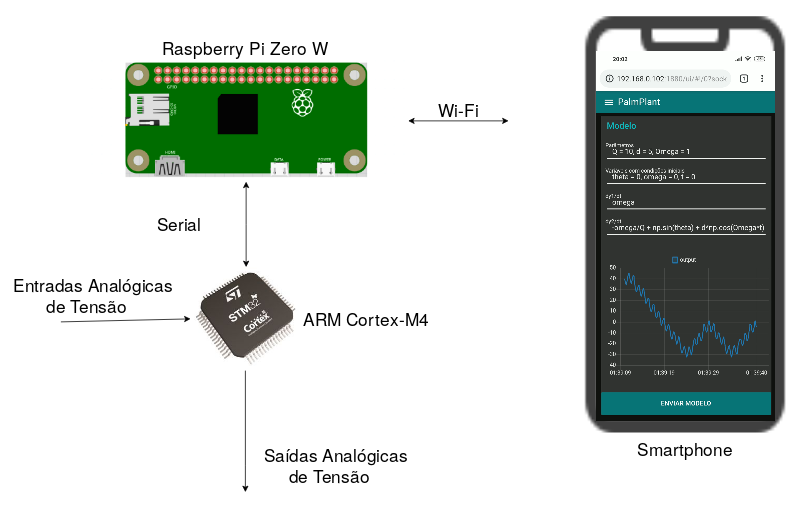
\includegraphics[width=\linewidth]{img/diagrama.png}
    \caption{Diagrama do Kit. Fonte: elaborado pelo autor}
    \label{fig:real}
\end{figure}

Como podemos ver, o elementos são poucos e as interfaces já bem conhecidas, ficando a cargo da camada de software implementar o diferencial desse projeto, que será explicado na sequência.

\subsection{Software}

O desenvolvimento do software pode ser dividido em três parte: servidor web, software em Python e o software para o microcontrolador. Esses itens serão explicados na sequência.

O servidor web é o principal contato do usuário com o kit, onde facilmente devem estar organizadas as informações, possibilidade de se enviar um modelo e visualizar o resultado da solução desse modelo. Para o desenvolvimento do mesmo, optamos pelo desenvolvimento em Node-Red, que é uma ferramenta para o desenvolvimento de dashboards de forma mais simples e direta, nos abstraindo todo o trabalho de se criar telas em HTML e scripts em JavaScript para gerencia-las. Esse servidor web é executado na própria RasPi Zero, o smartphone ou outro dispositivo com navegador, simplesmente recebe os dados e renderiza na pela o que o servidor está enviando. A imagem da sequência representa a tela inicial da interface com o usuário, onde temos alguns exemplos de modelos.

\begin{figure}[H]
	\centering
	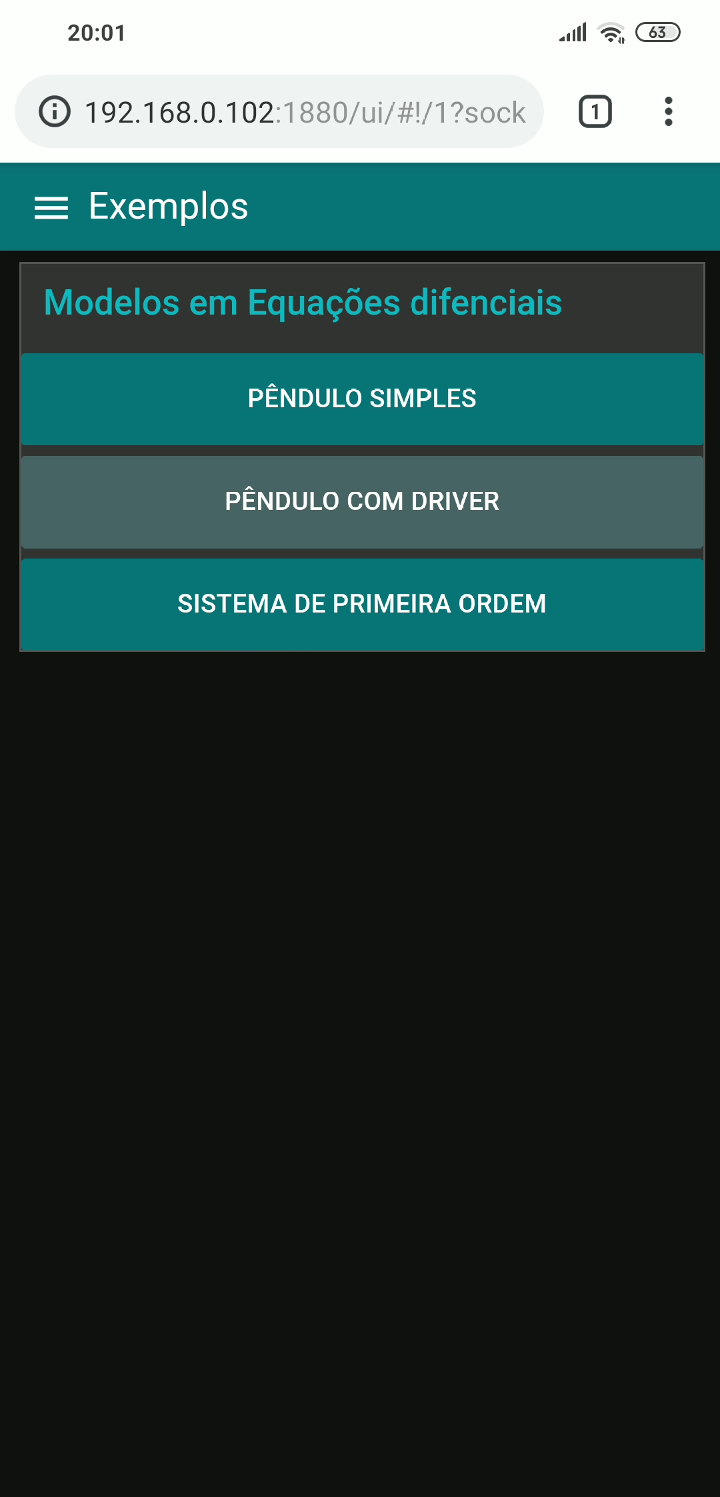
\includegraphics[width=4.1cm]{img/examples.png}
    \caption{Tela com exemplos de modelos. Fonte: elaborado pelo autor}
    \label{fig:examples}
\end{figure}

Já na próxima imagem, já podemos ver a tela para inserção ou configuração do modelo, que ainda permite visualizar o resultado das equações diferenciais.

\begin{figure}[H]
	\centering
	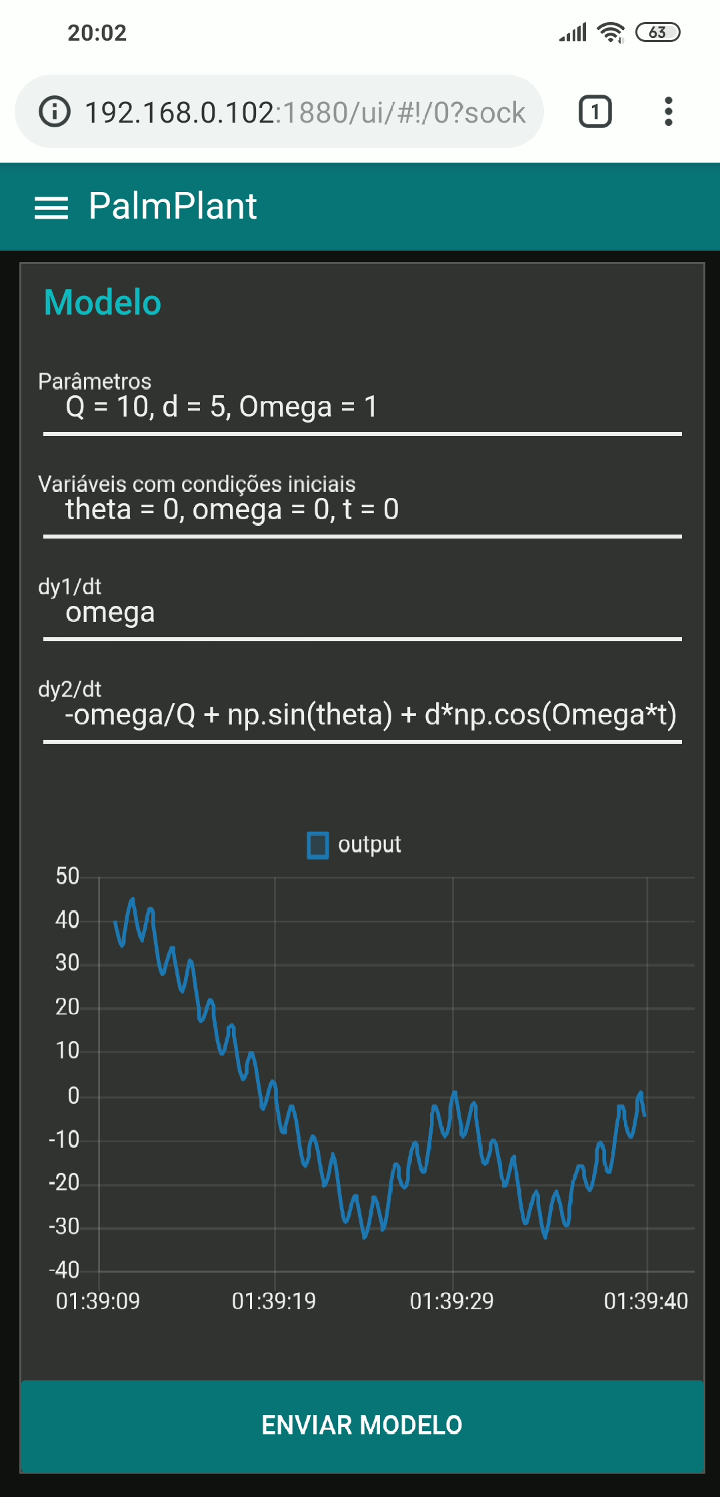
\includegraphics[width=4.1cm]{img/running.png}
    \caption{Tela de edição dos modelos e visualização da solução. Fonte: elaborado pelo autor}
    \label{fig:running}
\end{figure}

O software em Python é responsável por gerenciar a demanda de resolver o modelo requisitado pela interface de usuário, montar o modelo a partir dos dados recebidos da interface, resolver o modelo, enviar para a interface de usuário a resposta e enviar via serial o mesmo resultado para o microcontrolador, além de tratar outras interrupções que podem ser ativadas pelo usuário. Esse código é executado na RasPi Zero, juntamente com o servidor web.

O firmware que é executado no microcontrolador é simplificado, implementado em C, o qual recebe via serial o valor ele deve escrever nos ADCs, e também, lê os valores de tensão que estão nos DACs e envia via serial para a RasPi Zero. Todas as funções também são chamadas via interrupção, não travando o código em repetidas verificações.

O diagrama a seguir, representa as principais partes do software, onde o firmware do microcontrolador não está incluso, por ser muito simples.

\begin{figure}[H]
	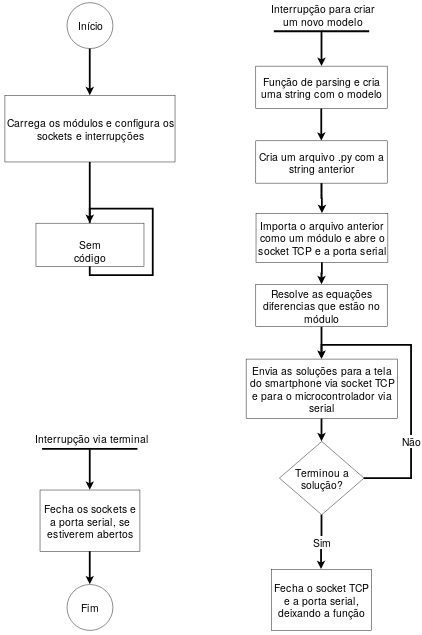
\includegraphics[width=\linewidth]{img/software.png}
    \caption{Diagrama de Software. Fonte: elaborado pelo autor}
    \label{fig:real}
\end{figure}

Com o diagrama anterior, concluímos o desenvolvimento e com isso, os resultados pode ser descrito.

%%%%%%%%%%%%%%%%%%%%%%%%%%%%%%%%%%%%%%%%%%%%%%%%%%%%%%%%%%%%%%%%%%%%%%%%%%%%%

\section{Resultados}

Como mostrado no desenvolvimento, a interface de usuário possui uma aba para inserção do modelo. Foi exatamente o que foi feito para se obter os resultados, inclusive o mesmo modelo que pode ser visto na figura \ref{fig:running}. A imagem a seguir representa o resultado do kit.

\begin{figure}[!h]
	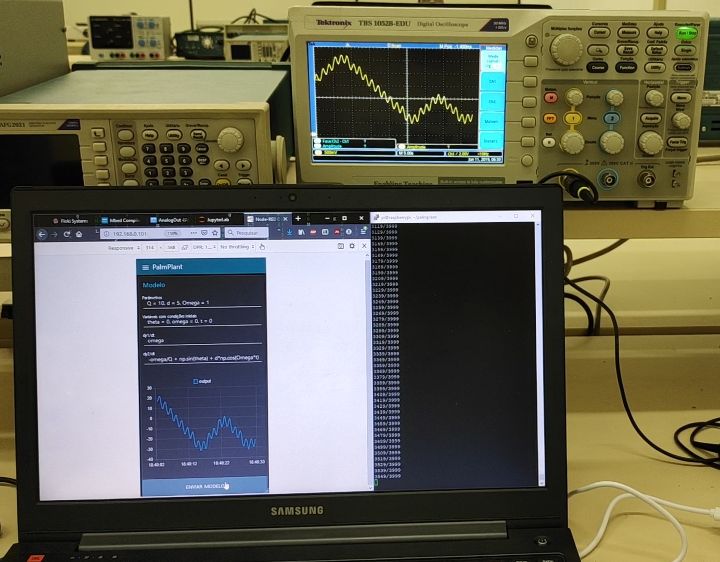
\includegraphics[width=\linewidth]{img/real_running.png}
    \caption{Funcionamento da saída analógica de tensão. Fonte: elaborado pelo autor}
    \label{fig:real}
\end{figure}

Como podemos ver, o mesmo gráfico que está presente na interface de usuário (laptop), também é vista no canal do osciloscópio, em tempo real com um tempo de atualização dos valores a cada \SI{50}{\milli\second}


%%%%%%%%%%%%%%%%%%%%%%%%%%%%%%%%%%%%%%%%%%%%%%%%%%%%%%%%%%%%%%%%%%%%%%%%%%%%%

\section{Conclusão}

O hardware se mostrou suficiente para essa aplicação, apresentado lentidão na RasPi Zero apenas em momentos que o tempo de atualização era menor do que \SI{40}{\milli\second}, o que poderia descaracterizar o sinal de saída.

As implementações dos softwares se mostraram eficazes, pois em nenhum momento a interface de usuário travou, apenas um atraso na atualização dos pontos da solução. Isso se deve as funções que implementam os gŕaficos, que não foram projetados para sinais que estão em na faixa de 50 ms de atualização, sendo mais usadas para sinais na faixa de segundos.

A funcionalidade geral do kit se mostrou muito promissora, onde em bancada, o kit conseguiu processar as entradas do usuário, resolver as equações diferenciais, enviar esses dados de volta para a interface do usuário, e externar esse sinal via um ADC, sendo visualizado simultaneamente no osciloscópio e na interface com o usuário.

Como um trabalho futuro, é imprescindível o projeto de uma placa de circuito impresso para unir todo o hardware em um único produto. Expandir a interface gráfica, criando telas para mais exemplos, outra para logs de sistemas e permitir o cascateamento dos kits, possibilitando a criação de um sistema mais complexo.

%%%%%%%%%%%%%%%%%%%%%%%%%%%%%%%%%%%%%%%%%%%%%%%%%%%%%%%%%%%%%%%%%%%%%%%%%%%%%

 \section{Bibliografia}

[1] E. A. Vendrusculo, A. A. Ferreira, J. A. Pomilio, “Plataforma Didática para Avaliação Rápida e Experimental de Estratégias de Controle em Eletrônica de Potência”; Eletrônica de Potência, vol. 13, no. 2, pp. 99-108, May 2008.

[2] Nise, Norman. Engenharia de Sistemas de Controle, 5. ed. editora LTC, 2011

\end{document}
